\section{Wetter-API(Datenquelle)}
In diesem Kapitel wird auf die im Rahmen dieses Projektes Wetter-API vom Anbieter "OpenWeatherMap" eingegangen und anschließend eigens dafür implementierte Services zu dieser beschrieben. Anschließend werden die für den Services implementierten Klassen, Methoden und Tests beschrieben. Abschließend wird diese Komponente gegen die zu Beginn definierten Anforderungen validiert. 
\subsection{Die API}
Der Anbieter "OpenWeatherMap" bietet kostenlos die Möglichkeit Wetterdaten via HTTP-Request abzufragen. 
Hierzu ist lediglich ein Nutzerzugang erforderlich, welchen sich jeder anlegen kann. Es können verschiedene Vorhersagen abgefragt werden, für diese Arbeit beschränkt es sich jedoch auf die tägliche Vorhersage und eine  5-tages Vorhersage. Solch ein angesprochener HTTP-Request (hier für eine 5-tägige Vorhersage) setzt sich wie folgt zusammen, 
\begin{lstlisting}
http://api.openweathermap.org/data/2.5/forecast?zip=78467,de&
APPID=41c464d95d33fabc24d44a5086ea9848
\end{lstlisting}

Der Parameter "ZIP" wird zum setzten der Postleitzahl für die gewünschte Stadt genutzt, zu diesem muss noch das Länderkürzel hinzugefügt werden. Die "APPID" wird von "OpenweatherMap" für jeden Nutzeraccount spezifisch vergeben und dient als Authentifizierung. Der Parameter"forecast" dient zur Unterscheidung zwischen einer aktuellen Vorhersage und einer 5-tages Vorhersage, bei Erster würde der Request wie folgt aussehen, 

\begin{lstlisting}
http://api.openweathermap.org/data/2.5/weather?zip=78467,de&
APPID=41c464d95d33fabc24d44a5086ea9848
\end{lstlisting}

hier muss lediglich der Parameter "forecast" durch "weather" ersetzt werden. 

"OpenWeatherMap" unterscheidet das Angebot zwischen kostenfrei und kostenpflichtig. Innerhalb der kostenpflichtigen Varianten gibt es Staffelungen, das gesamte Angebot wird aus Abb. \ref{img:OpenWeather} genauer ersichtlich. 

Für die in dieser Arbeit beschriebenen Lösung wurde auf die kostenfreie Variante gesetzt. Daher musste bei der Implementierung auf einige Einschränkungen geachtet werden, zu diesen gehören, 
TODO erkläre die Einschränkungen
\begin{itemize}
\item "Calls per minute (no more than)",
\item "Availibilty",
\item "Weather API data update".
\end{itemize}

Da auf das kostenfreie Modell gebaut wird, muss vor allem auf die erstgenannte Einschränkung (Abb. \ref{img:OpenWeather}) geachtet werden. Laut dieser sind lediglich 60 Requests mit den oben gezeigten URLs erlaubt. Im Rahmen der gesamten Anwendung wurde entscheiden, dass diese Applikation für alle Hauptstädte der 16 Bundesländer und Konstanz zur Verfügung stehen soll. Somit errechnet sich der Anteil an Requests pro Minute wie folgt,

\begin{align}
RequestsPerMin. = (16*2)+(2*2)\\
RequestsPerMin. = 36
\end{align}
somit kann ohne auf Probleme zu stoßen, ein Request-Intervall von 60 Sekunden, gewählt werden. 

\begin{figure}[!ht]
	\centering
	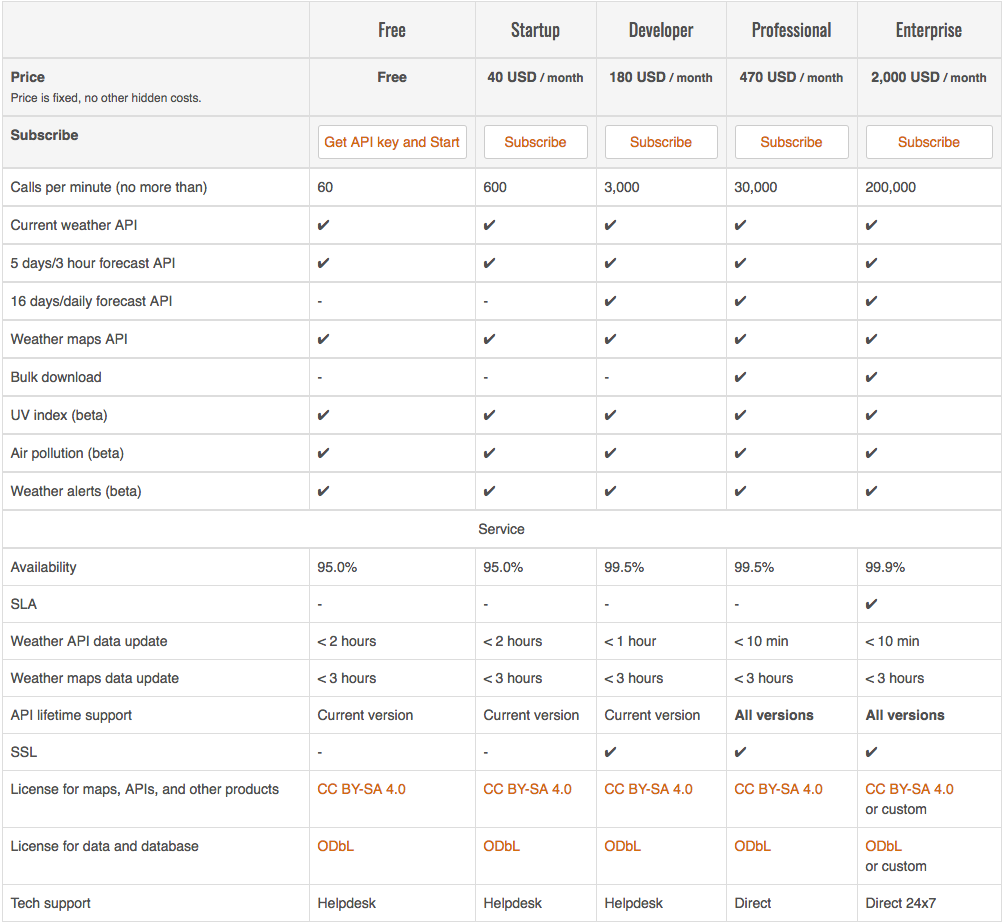
\includegraphics[width=1.0\textwidth]{Bilder/OpenWeatherMap.png}
	\caption{OpenWeatherMap Konditionen}
	\label{img:OpenWeather}
\end{figure} 
Im Bezug auf den "Response-Type" der API, kann entschieden werden, ob als "Response-Type" das JSON- oder XML-Format gewählt werden soll. Aufgrund der guten Möglichkeiten von Java mit JSON-Dokumente zu arbeiten, wurde  das JSON-Format, als "Response-Type", gewählt.
Um bessere Vorstellungen von solch einem Response im JSON-Format zu bekommen wird dieser untenstehend am Beispiel einer täglichen Vorhersage gezeigt.  

  \begin{lstlisting}
{"coord":{"lon":9.16,"lat":47.67},"weather":[{"id":800,"main":"Clear","description":"clear sky","icon":"01d"}],"base":"stations","main":{"temp":297.6,"pressure":1021,"humidity":41,"temp_min":296.15,"temp_max":298.15},"visibility":10000,"wind":{"speed":5.7,"deg":30},"clouds":{"all":0},"dt":1497797400,"sys":{"type":1,"id":4915,"message":0.0038,"country":"DE","sunrise":1497756293,"sunset":1497813872},"id":0,"name":"Konstanz","cod":200}
\end{lstlisting}

Des weiteren wird am nächsten Beispiel der Response-Type für die 5-tägige Vorhersage aufgezeigt, jedoch wird hier aufgrund des hohen Umfangs nur ein kleiner Teil (für 3 Stunden) gezeigt. Im Normalfall besteht ein vollständiger Response aus im 3 stunden Takt 
folgenden Informationen für 5 Tage.
 
  \begin{lstlisting}
{"cod":"200","message":0.0035,"cnt":40,"list":[{"dt":1497808800,"main":{"temp":295.56,"temp_min":294.226,"temp_max":295.56,"pressure":957.98,"sea_level":1034.02,"grnd_level":957.98,"humidity":53,"temp_kf":1.34},"weather":[{"id":800,"main":"Clear","description":"clear sky","icon":"01d"}],"clouds":{"all":0},"wind":{"speed":2.46,"deg":51.5021},"sys":{"pod":"d"},"dt_txt":"2017-06-18 18:00:00"}
\end{lstlisting}
\clearpage
Um mit diesen JSON-Response-Types besser und freier arbeiten zu können wurde ein Service implementiert, welche die Daten vorher Filtert, somit werden nur wichtige Informationen genutzt. Die Implementierung dieses Services wird im folgenden Abschnitt beschrieben. Der Service greift die Grundlagen und Problemstellungen der "OpenWeatherMap"-API auf, welche in diesem Abschnitt beschrieben wurden, von den Request-Intervallen bis hin zu den zwei verschiedenen Arten von Vorhersagen.

\subsection{Die Komponenten und Klassen}

Im untenstehenden Diagramm Abb.\ref{img:KomponentenWetterAPI} werden die einzelnen Teilkomponenten der in diesem Kapitel beschrieben Wetter-API sowie den zur Behebung des erläuterten RabbitMQ-Problems zusätzlich implementierten Komponenten gezeigt.

\begin{figure}[!ht]
	\centering
	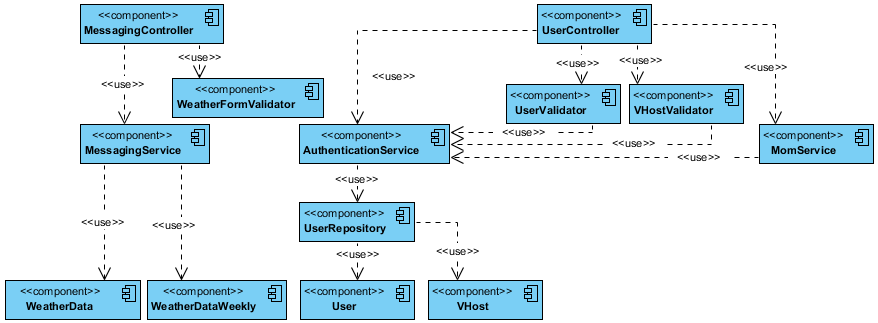
\includegraphics[width=1.0\textwidth]{Bilder/WetterApiKomponentendiagramm.PNG}
	\caption{Wetter-API Komponenten}
	\label{img:KomponentenWetterAPI}
\end{figure} 

Die zugrundeliegenden Klassen der einzelnen Komponenten werden im folgenden kurz beschrieben. Anschließend wird in den nächsten Abschnitten auf die wichtigsten Klassen und die darin enthaltenen Methoden noch genauer eingegangen. 

\begin{description}


\item[MessagingController:]Diese Klasse nimmt die Aufrufe der Wetterformulare der Startseite entgegen und leitet sie an den MessagingService weiter

\item[UserController:]Der User-Controller enthält die REST-Schnittstellen für den Login, die Registrierung neuer Nutzer und die Vergabe von Rechten. 
\item[User:]Die Userklasse beinhaltet die Attribute zur Persistierung und Verwaltung der Nutzerdaten.
\item[VHost:] Die Klasse VHost enthält den Namen des virtuellen Hosts, den Namen des Nutzers dessen Rechte geändert werden sowie die Ausprägung der Rechte, unterteilt in Lese-, Schreib- und Konfigurationsrechte.
\item[WeatherData:]Die Klasse dient als Grundlage für die Datenstruktur der täglichen Daten des JSON-Reponse, welche von der Klasse WeatherAPIService an die MOM gesendet werden. 
\item[WeatherDataWeekly:]Die Klasse dient als Grundlage für die Datenstruktur der wöchentlichen Daten des JSON-Reponse, welche von der Klasse WeatherAPIService an die MOM gesendet werden. 
\item[AuthenticationService:]Diese Klasse dient dem Aufruf der notwendigen Methoden im UserRepository.
\item[UserRepository:]Über das UserRepository erfolgt der Zugriff auf die hinterlegte Datenbank.
\item[WeatherApiService:]Die Klasse vom Typ MessagingService regelt die HTTP-Requests an die "OpenWeatherAPI" und ließt die HTTP-Responses aus, diese Klasse wird im nächsten Abschnitt noch genauer eingeführt, da sie essentiell ist. 

\item[MomService:]Über den MomService erfolgt der Zugriff auf die HTTP-API von RabbitMQ.
\item[SecurityService:]Durch den SecurityService wird der Name des eingeloggten Nutzers ermittelt.

\item[UserDetailsService:]Der UserDetailService ist eine Klasse von Spring Security und lädt einen User und seine Rechte.

\item[UserValidator:]Mit Hilfe des UserValidators erfolgt die Validierung des Registrierungsformulars auf ungültige Passwörter und bereits vorhandene Nutzernamen.
\item[VHostValidator:]Durch den VHostValidator werden die Eingaben im Formular zur Vergabe von Rechten validiert. 
\item[WeatherFormValidator:]Der WeatherFormValidator überprüft, ob alle notwendigen Eingaben zur Erstellung eigener Wetterdaten vorhanden sind.
\item[WeatherApiApplication:]Diese Klasse ist die Startklasse der Spring-Boot Applikation und lädt die properties-Dateien welche die Nachrichten der verschiedenen Validierungsklassen enthalten.
\item[WebSecurityConfig:]In dieser Klasse wird definiert, auf welche URLs dieser Anwendung ohne gültigen Login zugegriffen werden kann.

\end{description}

\subsubsection{Wetter-API-Service}

Für den Zugriff und die Abfrage der "OpenWeatherMap“-API wurde ein Service mit der Klasse "WeatherDataService" implementiert, welcher die Abfrage regelt und ein JSON mit der gewünschten Struktur zurückliefert. Dieses JSON wird dann mit Hilfe von "MQTT" an die MOM (vgl. Kap.\ref{rabbitmq}) gepublished. 

Die gesamte Komponente verfügt über einen Web-Client. Dieser Web-Client stellt die Möglichkeit bereit Testdaten an die MOM zu senden oder aber die Abfrage der Wetterdaten an die "OpenWeatherMap"-API zu starten. Da für die gesamte Applikation die Livedaten von grundlegender Wichtigkeit sind, muss dieser Service zu jeder Zeit laufen. Es ist im Realbetrieb nicht vorgesehen, dass dieser gestoppt wird.

Nachfolgend werden die wichtigsten Methoden der Klasse "WeatherDataService" beschrieben. 

\begin{description}
\item["init()"] füllt eine HashMap mit allen gewünschten Postleitzahlen auf, nach welchen die "OpenWeatherMap"-API abgefragt werden soll.
\item["public void publishLiveWeatherData()"] ruft im Intervall von 60 Sekunden die Methoden "handlePLZtoday(plz, countryCode)“ und „handlePLZweekly(plz, countryCode)“ mit allen Postleitzahlen und Countrycodes auf, welche in der Init() -Methode eingelesen wurden. 
\item["public void handlePLZtoday(String plz, String countryCode)"] stellt einen HTTP-Request und fragt die tagesaktuellen Wetterdaten im JSON-Format ab.
\item["public void dailyToWeatherData(...)"] liest den von der Methode "handlePLZtoday" gestellten HTTP-Request aus und zieht die gewünschten Daten anhand der Struktur der Klasse "WeatherData" aus dem Response-JSON der "OpenWeatherMap"-API. Anschließend wird  die gewünschte JSON-Struktur zusammengebaut. 
\item["public void handlePLZweekly(String plz, String countryCode)"]stellt einen HTTP-Request und fragt die 5-tägigen Wetterdaten im JSON-Format ab.
\item["public static ArrayList WeatherDataWeekly weeklyToWeatherDataWeekly 
(...)" ]liest den von der Methode "handlePLZweekly" gestellten HTTP-Request aus und zieht die gewünschten Daten anhand der Struktur der Klasse "WeatherDataWeekly" aus dem Response-JSON der "OpenWeatherMap"-API. Anschließend wird die gewünschte JSON-Struktur zusammengebaut.
\item["private void reconnectToMoM()"] stellt sicher, dass bei einem Verbindungsverlust zur MOM wieder eine Verbindung hergestellt wird. 
\item["public void publishFakeWeatherData(WeatherData weatherData)"] sendet die Daten, via Web-Client eingepflegt wurden, an die MOM. 
\end{description}

Im nachfolgenden Abschnitt wird die Implementierung zur Lösung des in Absatz \ref{rabbitmq} erläuterten Problems beschrieben. Dafür wurde ein Registrierungs- und Rechtevergabeprozess implementiert. Auf Grundlage der dabei erstellten Datensätze wird zum Abschluss eines Registrierungsprozesses oder der Vergabe von Rechten das init.sh Shellskript erstellt. Dieses kann dem Dockerimage hinzugefügt werden und legt beim Start eines Containers automatisch die Nutzer in RabbitMQ an.
Damit der Zugriff auf die Registrierungs- und Rechteseite auf den Administrator beschränkt ist, wird dies in der Klasse WebSecurityConfig so definiert. In der selben Klasse werden auch die REST-Schnittstellen definiert die ohne Authentifizierung erreichbar sind. Ruft der Nutzer eine Schnittstelle auf, für die eine Authentifizierung oder eine andere Rolle notwendig ist, erscheint ein Login-Fenster. Die REST-Schnittstellen für den Login und die Rechtevergabe der virtuellen Hosts erfolgt über den UserController. Im UserController erfolgt die Persistierung und Validierung der Daten mit der in Kapitel 5 erläuterten Datenbank durch den Authentifizierungsservice. Gleichzeitig werden die Daten dieser Nutzer über die HTTP-API von RabbitMQ in selbigem gespeichert. Dies erfolgt durch den MomService.
\subsubsection{Authentifizierungsservice}\label{momservice}
Der Authentifizierungsservice wird über den UserController aufgerufen. Der Service selbst wird für den Login-Prozess, die Registrierung neuer Nutzer und die Rechtevergabe für die virtuellen Hosts aufgerufen. Der Login-Prozess wird dabei vollständig von Spring Security übernommen. Wird ein neuer Nutzer registriert, erfolgt zuerst die Validierung der eingebenen Daten durch den UserValidator. Dabei wird geprüft, ob der Nutzer bereits vorhanden ist und das Passwort mit dem Bestätigungspasswort übereinstimmt. Bei einer fehlerhaften Eingabe oder einem bereits vorhandenen Nutzer wird die entsprechende Ausgabe auf der Weboberfläche ausgegeben. War die Validierung erfolgreich, wird die Methode createUser(userForm) aufgerufen. Diese ruft die Methode insertSystemUser(Username, encodedPassword, Description) auf. Die Verschlüsselung des Passworts erfolgt über den BCryptPasswordEncoder von Spring Security. Im UserReposity werden die notwendigen SQL Statements aufgerufen, um den Nutzer in der Datenbank zu sichern. Die Vergabe von Rechten für virtuelle Hosts erfolgt über die Methode addPermission(vHostForm) des Authentifizierungsservices. Die vHostForm wird vorab durch den VHostValidator geprüft, ob der zugewiesene Nutzer bereits existiert. Anschließend erfolgt der Aufruf der addPermission-Methode und die Speicherung der Rechte des Nutzers für den virtuellen Host in der Datenbank über das UserRepository.
\subsubsection{MOM-Service}
Neben den Speicherung der Nutzer und Berechtigungen in der Datenbank müssen diese ebenfalls im RabbitMQ gespeichert werden. Dies erfolgt im MOM-Service. Der Service enthält dazu die Methoden addUser(loggedInUser, userToSave), setPermission(loggedInUser, userToSave, vHost) und createVHost(loggedInUser, vHost). Diese Methoden greifen über definierte Schnittstellen der HTTP-API auf RabbitMQ zu. Die Variable loggedInUser wird benötigt, um mit dessen Zugangsdaten über einen curl-Request die notwendigen Schnittstellen aufzurufen. Dies ist nur möglich, wenn der eingeloggte Nutzer Administrator-Rechte auf der RabbitMQ-Instanz hat. Zusätzlich enthält der MOM-Service die Methode writeScript(). Durch diese Methode werden die aktuellen Nutzer und ihre Rechte aus der Datenbank geladen und als rabbitmqctl-Aufruf im init-Skript für das Containerimage gespeichert. Das Skript kann in ein Repository für das Containerimage gespeichert werden. Beim der Ausführung des Dockerfiles  wird das Skript als Startpunkt für den Container definiert. Wird der Container gestartet, erfolgt die Ausführung des Skripts und die Nutzer werden gemeinsam mit den aus der Datenbank ermittelten Berechtigungen beim Start des Containers angelegt. Auf das Deployment des Dockercontainers wird in Absatz \ref{Docker} noch genauer eingegangen.




%\subsection{Testing}
%Im Rahmen des Testings wurde für die Klasse "WeatherAPIService" eine Testklasse "WeatherAPIServiceTest" angelegt. 
%Diese Klasse testet die wichtigsten Methoden der Ursprungsklasse, zu den Testmethoden gehören,

%\begin{itemize}
%\item "testAPICallTodayWithoutWindDeg()"
%\item "testAPICallTodayWithWindDeg()"
%\item "testAPICallWeeklyWithoutWindDeg()"
%\item "testAPICallWeeklyWithWindDeg()"
%\end{itemize}

%Die ersten zwei Methoden Testen, für den Fall eines HTTP-Response seitens der API für eine tagesaktuelle Wettervorhersage. Dafür wurde ein String mit gefakten Daten angelegt, mit diesen Daten wurde dann die Methode "dailyToWeatherData" aufgerufen, somit kann sichergestellt werde, dass die endgültige Form des JSON mit der gewünschte der "WeatherData" Klasse übereinstimmt. 
%Hier muss jedoch eine Fallunterscheidung gemacht werden, da in der Methode noch mit Hilfe einer Kontrollstruktur der Fall %angefangen wird, dass die API für die Windrichtung keinen Wert sendet. Dieser Fall tritt immer dann ein, wenn die Windstärke unter den Wert 1.5 sinkt. Aus diesem Grund gibt es, wie oben angegeben, diese zwei Fallunterscheidung bei den Testmethoden. 

%Die weiteren zwei Methoden testen einen fast anlogen Fall zu den ersten zwei ab nur das hier ein HTTP-Response für eine 5-tägige Wettervorhersage getestet wird. Der unterschied besteht in der Konstruktion der Testdaten, da diese eine komplexere und größere Menge aufweisen, als in den ersten beiden Fällen. Aus dem Grund wurden 2 Hilfsmethoden implementiert, welche einen String bauen, welcher gleich einem API-Response für eine 5-tägige Vorhersage ist.

\subsection{12 Faktor App}\label{12FactorAppWeatherAPI}

\begin{table}[!ht]
  \centering
    \begin{minipage}{15cm}
      \centering
      \begin{tabular}{*{3}{|l|p{5.0cm}|p{5.0cm}}}\hline
      \multicolumn{4}{|c|}{\cellcolor[RGB]{200,200,200}Validierung nach "12 Faktor APP"} \\\hline
     \textbf{ID}&\textbf{Anforderung}&\textbf{Validierungs Element}&\textbf{Erfüllt}\\\hline
     1.&Codebase&Andere Komponenten sind nur für das Testszenario da. Deployment verschiedener Versionen über Repo möglich&Ja\\
      \hline
     2.&Abhängigkeiten&Zugriff auf die Datenbank und die "OpenWeatherMap"-API sind in eigenen Klassen isoliert&Ja\\
     \hline
     3.&Konfiguration&Credentials werden über Umgebungsvariablen im Jenkings-Server verwaltet&Ja\\
     \hline
     4.&Unterstützende Dienste&Credentials der "OpenWeatherMap"-API werden über die Umgebungsvariablen im Jenkins-Server verwaltet&Ja\\
     \hline 
     5.&Build, release, run&Wird über einen Jenkins-Server verwaltet&Ja\\
     \hline
     6.&Prozesse&Wird via Web-Gui gestartet&Ja\\
     \hline
      7.&Bindung an Ports&Die Ports werden von Pivotal verwaltet&Ja\\
     \hline
     8.&Nebenläufigkeit&Es könnte zu jeder Zeit eine neue Instanz auf Pivotal gestartet werden, jedoch bedarf es bei dieser Komponente keiner Skalierung&Ja\\
     \hline
      \end{tabular}
   \caption{Validierung nach "12 Faktor APP"}\label{tab:Anforderungen}
    \end{minipage}
\end{table}

\begin{table}[!h]
  \centering
    \begin{minipage}{15cm}
      \centering
      \begin{tabular}{*{3}{|l|p{5.0cm}|p{5.0cm}}}\hline
      \multicolumn{4}{|c|}{\cellcolor[RGB]{200,200,200}Validierung nach "12 Faktor APP"} \\\hline
     \textbf{ID}&\textbf{Anforderung}&\textbf{Validierungs Element}&\textbf{Erfüllt}\\\hline

      9.&Einweggebrauch&Pivotal generiert aus der hochgeladenen .jar oder .war einen Container, welcher jeder Zeit über die GUI in Pivotal gestoppt werden kann. &Ja\\
     \hline
     10.&Dev-Prod-Vergleichbarkeit&Containerisierung durch Pivotal&Ja\\
     \hline     
     11.&Logs&Pivotal gibt die Logs standardmäßig über Stdout aus&Ja\\
     \hline
     12.&Admin-Prozesse&Nicht vorhanden&Nein\\
     \hline
      \end{tabular}
   \caption{Validierung nach "12 Faktor APP"}\label{tab:Anforderungen}
    \end{minipage}
\end{table}